%\newcommand{\filespath}{../../Style/}%  JANCL path

\documentclass[french,utf8]{./hermes-journal}
\usepackage[frenchb]{babel}
\usepackage[utf8]{inputenc}
\usepackage[T1]{fontenc}
% \journalName{year}{volume}{issue}
\ria{2013}{27}{2}
\firstpagenumber{155}
%\lastpagenumber{179}
\let\chapter\section
\usepackage[ruled,algo2e,french]{algorithm2e}
\usepackage{mathtools}
\usepackage{subfigure}
\usepackage{gensymb}
\mathtoolsset{showonlyrefs=true}

\newcommand{\argmax}{\operatorname*{argmax}} %\operatorname* pour les op. pouvant admettre des limites...
\newcommand{\argmin}{\operatorname*{argmin}}
\newcommand{\diag}{\operatorname*{diag}}

\newcommand{\p}{\mathcal{P}}
\newcommand{\R}{\mathcal{R}}
\newcommand{\s}{\mathcal{S}}
\newcommand{\A}{\mathcal{A}}
\newcommand{\X}{\mathcal{X}}
\newcommand{\Y}{\mathcal{Y}}
\newcommand{\D}{\mathcal{D}}
\newcommand{\T}{\mathcal{T}}
\newcommand{\lc}{\mathcal{L}}
\newcommand{\E}{\mathbb{E}}
\newcommand{\prob}{\mathbb{P}}
\newcommand{\Mu}{\boldsymbol{\mu}}
%\newcommand{\Xi}{\boldsymbol{\xi}}


%\newtheorem{theorem}{Theorem}

% \title[short header title]{title}
\title[SCIRL]{Classification structurée pour l'apprentissage par renforcement inverse}
\author[1,2]{Edouard}{Klein}
\author[2,3]{Bilal}{Piot}
\author[2]{Matthieu}{Geist}
\author[2,3]{Olivier}{Pietquin}


% addresses are automatically numbered
\address{LORIA -- équipe ABC\\
Nancy, France
\vspace{-2em}
}{}
\address{Supélec -- Groupe de recherche IMS-MaLIS\\
Metz, France}
        {prenom.nom@supelec.fr}
\address{ UMI 2958 (GeorgiaTech-CNRS)\\
Metz, France
\vspace{-2em}
}{}

\abstract{  This paper adresses the inverse reinforcement learning (IRL) problem, that
  is inferring a reward for which a demonstrated expert behavior is
  optimal. We introduce a new algorithm, SCIRL, whose principle is to use
  the so-called feature expectation of the expert as the
  parameterization of the score function of a multiclasse
  classifier. This approach produces a reward function for which the
  expert policy is provably near-optimal. Contrary to most of
  existing IRL algorithms, SCIRL does not require solving the
  direct RL problem. Moreover, with an appropriate heuristic, it can succeed with only trajectories sampled
  according to the expert behavior. This is illustrated on a car
  driving simulator.}
\resume{Cette contribution traite le problème de l'apprentissage par renforcement inverse (ARI), défini comme la recherche d'une fonction de récompense pour laquelle le comportement d'un expert (connu par le biais de démonstrations) est optimal. Nous introduisons SCIRL, un nouvel algorithme qui utilise la grandeur dénommée attribut moyen de l'expert comme la paramétrisation d'une fonction de score pour un classifieur multiclasse. Cette approche donne une fonction de récompense pour laquelle la politique de l'expert est (nous le démontrons) quasi optimale. Contrairement à la plupart des algorithmes d'ARI existants, SCIRL n'a pas besoin de résoudre le problème direct de l'apprentissage par renforcement. De plus, en utilisant une heuristique, il fonctionne avec uniquement des trajectoires échantillonnées par l'expert. Nous illustrons cela sur un simulateur de conduite.}

\keywords{reinforcement learning, inverse reinforcement learning.}
\motscles{apprentissage par renforcement, apprentissage par renforcement inverse.}


\begin{document}
\maketitle

\newpage
\section{Introduction}
\label{sentro}

L'apprentissage par renforcement inverse (ARI) est le problème lié à la recherche, à partir de démonstrations d'un expert, d'une fonction de récompense telle que le comportement de l'expert soit optimal ; historiquement proposé dans~\cite{Russel998}, ce mécanisme trouve des applications dans divers champs, de la biologie à la neuropsychologie en passant par l'économie et plus récemment la robotique~\cite{abbeel2010autonomous}. Beaucoup d'algorithmes d'ARI (que nous décrirons succinctement section~\ref{seelatedWorks}) cherchent une fonction de récompense dont la politique optimale associée génère une distribution sur les trajectoires (ou une grandeur liée à cette distribution) proche de celle générée par l'expert. Souvent, cette distribution est caractérisée par ce que l'on appelle l'attribut moyen (voir section~\ref{subseackgrounrl}) : étant donnée une fonction de récompense linéairement paramétrée par un vecteur d'attributs, il s'agit de l'espérance de la somme pondérée des vecteurs d'attributs sachant que l'on commence dans un certain état en choisissant une certaine action avant de suivre la politique concernée.

Dans cette publication, nous choisissons une autre option. Il est possible d'imiter le comportement de l'expert via un algorithme d'apprentissage supervisé généralisant l'association des actions aux états. Nous considérons ici les classifieurs multiclasses qui à partir d'une base d'entraînement calculent les paramètres d'une fonction de score paramétrée linéairement ; la règle de décision pour un état est l'argument (l'action) qui maximise la fonction de score pour cet état (voir section~\ref{subseackgrounlassif}). L'idée de base de l'algorithme SCIRL que nous proposons est simplement d'estimer l'attribut moyen de l'expert comme la paramétrisation de la fonction de score (voir section~\ref{subsecirlgo}). Le vecteur de paramètres ainsi calculé définit une fonction de récompense dont on montre qu'elle admet pour politique quasi optimale la politique de l'expert (voir section~\ref{subsecirnalysis}).

Un grand avantage de SCIRL est qu'il ne requiert pas, contrairement à la plupart des algorithmes d'ARI, la résolution répétée du problème direct, celui de l'apprentissage par renforcement. Il nécessite d'estimer l'attribut moyen de l'expert, mais ceci est équivalent à un problème d'évaluation de la politique (pour une politique observée, ce qui est moins problématique que l'optimisation répétée d'une politique), voir section~\ref{seracticalApproach}.
De plus, à l'aide d'une heuristique, SCIRL peut s'éxécuter en utilisant uniquement des transitions issues de la politique de l'expert (il n'y a pas besoin d'échantillonner la dynamique complète). Nous illustrons cela sur un simulateur de conduite section~\ref{sexperiments}.

\section{Contexte et notations}
\label{seackground}

\subsection{Apprentissage par renforcement (inverse)}
\label{subseackgrounrl}

Un processus décisionnel de Markov (PDM)~\cite{Puterma994} est donné par le tuple $\{\s,\A,\p,\R,\gamma\}$ où $\s$ est l'espace d'état fini, $\A$ est l'espace d'action fini, $\p =
\{P_a = (p(s'|s,a))_{1\leq s,s'\leq |\s|}, a\in\A\}$ est l'ensemble des probabilités de transition markoviennes, $\R\in\mathbb{R}^\s$ est la fonction de récompense sur les états et $\gamma$ est le facteur d'oubli.
Une politique déterministe $\pi\in\s^\A$ définit le comportement d'un agent. La qualité de ce comportement est quantifiée par le biais de la fonction de valeur $v_\R^\pi\in\mathbb{R}^\s$, qui à chaque état associe la récompense pondérée cumulée moyenne recueillie par l'agent lorsqu'il part de cet état et suit la politique $\pi$ par la suite : $v_\R^\pi(s) = \E[\sum_{t\geq 0} \gamma^t \R(S_t)|S_0=s,\pi]$. Une politique optimale $\pi_\R^*$ (vis-à-vis de la fonction de récompense $\R$) est une politique dont la fonction de valeur $v^*_\R$ vérifie $v_\R^* \geq v_\R^\pi$ (composante par composante) pour toute politique $\pi$.

Soit $P_\pi$ la matrice stochastique définie par $P_\pi =
(p(s'|s,\pi(s)))_{1\leq s,s'\leq |\s|}$. Un léger abus de notation nous permet de nommer $a$ la politique associant l'action $a$ à chaque état $s$. Les opérateurs d'évaluation (respectivement d'optimalité) de Bellman $T^\pi_\R\text{ (resp. $T^*_\R$)}:\mathbb{R}^\s
\rightarrow \mathbb{R}^\s$ sont définis par $T^\pi_\R v = \R + \gamma
P_\pi v$ et $T_\R^*v = \max_\pi T_\R^\pi v$.
%\begin{equation}
%  T^\pi_\R v = \R + \gamma P_\pi v \text{ et } T_\R^*v = \max_\pi T_\R^\pi v.
%\end{equation}
Ces opérateurs sont des contractions qui admettent $v_\R^\pi$ et $v^*_\R$ comme points fixes respectifs : $v_\R^\pi = T^\pi_\R v_\R^\pi$ et $v^*_\R = T^*_\R v^*_\R$.
La fonction de qualité $Q^\pi\in\mathbb{R}^{\s\times \A}$ ajoute un degré de liberté dans le choix de la première action : $Q_\R^\pi(s,a)
= [T^a_\R v^\pi_\R](s)$. La distribution stationnaire de la politique $\pi$ est notée $\rho_\pi$, elle satisfait $\rho_\pi^\top P_\pi = \rho_\pi^\top$.

L'objectif de l'apprentissage par renforcement (AR) est d'estimer la politique de contrôle optimale lorsque le modèle (les probabilités de transition et la fonction de récompense) est inconnu (mais observé par interaction avec le système à contrôler) et quand l'espace d'état est trop grand pour qu'une représentation exacte des objets concernés (fonctions de valeur, politiques) soit possible~\cite{Bertseka996,Sutto998,szepesvari2010c}.
%
C'est le problème direct.
%
L'apprentissage par renforcement inverse (approché)~\cite{N000} consiste à estimer la fonction de récompense pour laquelle une politique observée est optimale.
%
Cette politique est la politique de l'expert, notée $\pi_E$. Elle est supposée optimale vis-à-vis d'une certaine fonction de récompense $\mathcal{R}_E$ inconnue. Le but de l'ARI est de calculer une fonction de récompense $\hat{\R}$ telle que la politique de l'expert soit (quasiment) optimale, c'est-à-dire telle que $v^*_{\hat{\R}}
\approx v^{\pi_E}_{\hat{\R}}$.
%
Nous appelons cela le problème inverse.

De la même manière que pour le problème direct, l'espace d'état peut être trop grand pour que la fonction de récompense admette une représentation exacte exploitable. La recherche est donc limitée à celle d'une bonne fonction de récompense paramétrée linéairement. Soit $\phi(s) = (\phi_1(s)  \dots
\phi_p(s))^\top$
%\begin{pmatrix}
%  \phi_1(s) & \dots & \phi_p(s)
%\end{pmatrix}^\top$
un vecteur d'attributs composé de $p$ fonctions de base $\phi_i\in\mathbb{R}^\s$, les fonctions de récompense paramétrées sont définies par $\R_\theta(s) = \theta^\top \phi(s) = \sum_{i=1}^p
\theta_i \phi_i(s)$.
%\begin{equation}
%  \R_\theta(s) = \theta^\top \phi(s) = \sum_{i=1}^p \theta_i \phi_i(s).
%\end{equation}
La recherche d'une bonne récompense est donc ramenée à la recherche d'un bon vecteur de paramètres $\theta \in\mathbb{R}^p$. Nous utiliserons indifféremment $\R_\theta$ et $\theta$ comme indices (\textit{e.g.}, $v_\theta^\pi$ pour $v_{\R_\theta}^\pi$).
Cette paramétrisation de la récompense implique une paramétrisation similaire de la fonction de qualité :
\begin{equation}
  Q^\pi_\theta(s,a) = \theta^\top \mu^\pi(s,a) \text{ avec }
  \mu^\pi(s,a) = \E[\sum_{t\geq 0} \gamma^t
  \phi(S_t)|S_0=s,A_0=a,\pi].
  \label{eeu}
\end{equation}
Conséquemment, la fonction de qualité partage son vecteur de paramètres avec la fonction de récompense, mais en relation avec un vecteur d'attributs $\mu^\pi$ appelé l'attribut moyen. Cette notion est de prime importance pour notre contribution. Chaque composante $\mu_i^\pi$ de ce vecteur d'attributs est en réalité la fonction de qualité de la politique $\pi$ pour la récompense $\phi_i$: $\mu_i^\pi(s,a) = Q^\pi_{\phi_i}(s,a)$. De fait, tout algorithme d'estimation de la fonction de qualité peut être utilisé pour estimer l'attribut moyen, comme une estimation de Monte-Carlo ou un algorithme aux différences temporelles~\cite{Klei011}.

\subsection{Classifieurs à fonction de score paramétrée linéairement} \label{subseackgrounlassif}

Soit $\X$ un ensemble fini ou compact (d'entrées à classifier)
 et soit $\Y$ un ensemble fini (de labels). Supposons que les entrées $x\in
\X$ sont tirées selon une distribution inconnue $\prob(x)$ et qu'il existe un oracle qui à chacune de ces entrées associe un label $y\in Y$ tiré selon une distribution de probabilité conditionnelle inconnue $\prob(y|x)$. De manière générale, la classification multiclasse cherche, étant donné une base d'entraînement $\{(x_i,y_i)_{1\leq i \leq N}\}$ tirée selon $\prob(x,y)$, une règle de décision $g\in\Y^\X$ minimisant l'erreur de classification $\E[\chi_{\{g(x)\neq y\}}] = \prob(g(x)\neq y)$, où $\chi$ est la fonction indicatrice.

Nous nous préoccupons ici d'un ensemble plus réduit de classifieurs. Nous supposons que la règle de décision associe à l'entrée l'argument qui maximise une certaine fonction de score, celle-ci étant paramétrée linéairement, les paramètres étant appris par le classifieur. Formellement, soit $\psi(x,y) =
(\psi_1(x,y)  \dots  \psi_d(x,y))^\top\in \mathbb{R}^d$
%\begin{pmatrix}   \psi_1(x,y) & \dots & \psi_d(x,y)
%\end{pmatrix}^\top \in \mathbb{R}^d$
un vecteur d'attributs dont les composantes sont $d$ fonctions de base $\psi_i\in\mathbb{R}^{\X\times\Y}$. La fonction de score linéairement paramétrée $s_w\in\mathbb{R}^{\X\times \Y}$ de vecteur de paramètres $w\in\mathbb{R}^d$ est définie par $s_w(x,y) = w^\top \psi(x,y)$. La règle de décision associée $g_w\in{\Y^\X}$ est définie par $g_w(x) \in \argmax_{y\in\Y}s_w(x,y)$. En se basant sur une base d'entraînement $\{(x_i,y_i)_{1\leq
i\leq N}\}$, un classifieur multiclasse (noté CMC) à fonction de score paramétrée linéairement choisit un vecteur de paramètres $\theta_c$. La qualité de ce choix est quantifiée par l'erreur de classification $\epsilon_c =
\prob(g_{\theta_c}(x)\neq y)$. %Riflette

Notre étude est valable pour tout algorithme de classification tant qu'il opère en maximisant l'argument d'une fonction de score paramétrée linéairement. Par exemple, un séparateur à vaste marge multiclasse pourrait être choisie~\cite{Guermeu007} (en considérant le noyau induit par le vecteur d'attributs) ou encore une approche à vaste marge structurée~\cite{Taska005}. 

\section{Classification structurée pour l'apprentissage par renforcement inverse} \label{secirl}

\subsection{Forme générale de l'algorithme}
\label{subsecirlgo}

Nous nous trouvons dans le cadre de la classification décrit en section~\ref{subseackgrounlassif}. L'entrée $x$ peut être vue comme un état et le label $y$ comme une action. Il s'ensuit que la règle de décision 
$g_w(x)$ est interprétable comme une politique gloutonne vis-à-vis de la fonction de score $w^\top \psi(x,y)$, qui peut elle-même être vue comme une fonction de qualité. Le parallèle avec l'équation~\eqref{eeu} est aisé, si $\psi(x,y)$ est l'attribut moyen d'une politique $\pi$ qui a fourni les labels de la base d'entraînement, et si l'erreur de classification est faible, alors $w$ est le vecteur de paramètres de la fonction de récompense vis-à-vis de laquelle on espère que la politique $\pi$ est quasi optimale. 
Ces remarques nous permettent maintenant d'introduire notre algorithme d'ARI par classification structurée (SCIRL pour \emph{Structured Classification-based Inverse Reinforcement Learning}).

Soit $\pi_E$ la politique de l'expert à partir de laquelle nous souhaitons inférer une fonction de récompense. Soit $\D = \{(s_i, a_i=\pi_E(s_i))_{1\leq i\leq N}\}$ une base d'entraînement où les états sont échantillonnés selon la distribution stationnaire de l'expert\footnote{Par exemple, si la chaîne de Markov induite par la politique de l'expert est à mélange rapide (\emph{fast-mixing}), l'échantillonnage d'une trajectoire donnera rapidement des échantillons tirés selon cette distribution.} $\rho_E = \rho_{\pi_E}$.
Supposons également avoir à disposition une estimée $\hat{\mu}^{\pi_E}$ de l'attribut moyen de l'expert $\mu^{\pi_E}$ défini à l'équation~\eqref{eeu}. Une description de la manière d'estimer cette quantité en pratique est reportée à la section~\ref{subseracticalApproacuE}; rappelons tout de même qu'estimer $\mu^{\pi_E}$ est simplement un problème d'\emph{évaluation de la politique} (estimation de la fonction de qualité d'une politique), comme signalé section~\ref{subseackgrounrl}. Supposons enfin qu'un algorithme de CMC a été choisi. L'algorithme formant notre contribution consiste simplement à choisir $\theta^\top\hat{\mu}^{\pi_E}(s,a)$ comme fonction de score paramétrée linéairement, puis à entraîner le classifieur sur $\D$, ce qui produit un vecteur de paramètres $\theta_c$, puis enfin à renvoyer la fonction de récompense $\R_{\theta_c}(s) = \theta_c^\top \phi(s)$.

\begin{algorithm2e}%[tbh]
    %\small
  \SetAlgoVlined
  \caption{{\it SCIRL}}
  \label{algcirl}
  %
  \BlankLine
  \emph{\textbf{Etant donnée}} une base d'entraînement $\D = \{(s_i,a_i=\pi_E(s_i))_{1\leq i\leq N}\}$,
  une estimée $\hat{\mu}^{\pi_E}$ de l'attribut moyen de l'expert $\mu^{\pi_E}$ et un algorithme de CMC\;
  %
  \BlankLine
  \emph{\textbf{Calculer}} le vecteur de paramètres $\theta_c$ en utilisant l'algorithme de CMC auquel sont fournis la base d'entraînement $\D$ et la paramétrisation de la fonction de score : $s_\theta(s,a) = \theta^\top\hat{\mu}^{\pi_E}(s,a)$\;
  %
  \BlankLine
  \emph{\textbf{Renvoyer}} la fonction de récompense $\R_{\theta_c}(s) = \theta_c^\top\phi(s)$ \;
\end{algorithm2e}

L'approche proposée est résumée par l'algorithme~\ref{algcirl}. Le nom de l'algorithme (SCI\-RL, que l'on peut traduire par Classification structurée pour l'ARI), vient de l'utilisation de l'attribut moyen de l'expert dans le classifieur, ce qui revient d'une certaine manière à prendre en compte la structure du MDP dans le problème de classification et permet le calcul du vecteur de paramètres de la récompense. Contrairement à la plupart des algorithmes d'ARI existants, SCIRL n'a pas besoin de résoudre le problème direct. Cet algorithme requiert une estimation de l'attribut moyen de l'expert mais il ne s'agit là que d'un problème d'évaluation de la politique, notoirement moins difficile que la recherche de politiques optimales qu'implique la résolution du problème direct. Cela est discuté plus en détail section~\ref{seelatedWorks}.
%
%Now, we formally show that the proposed approach makes sens, as long
%as $\mu^{\pi_E}$ is well estimated et as long as the classification
%error is small.


\subsection{Analyse}
\label{subsecirnalysis}

Dans cette section, nous montrons que la politique de l'expert $\pi_E$ est quasi optimale vis-à-vis de la fonction de récompense $\R_{\theta_c}$, plus précisément qu'il est possible de contrôler le terme
$\E_{s\sim\rho_E}[v^*_{\theta_c}(s)-v^{\pi_E}_{\theta_c}(s)]$.
Avant de présenter le résultat principal, il nous faut introduire quelques notations et définir quelques objets.

Nous allons utiliser le coefficient de concentration $C_f$~\cite{Muno007}:
\begin{equation}
  C_f = (1-\gamma)\sum_{t\geq 0} \gamma^t c(t) \text{ avec } c(t) =
  \max_{\pi_1,\dots,\pi_t,s\in\s}\frac{(\rho_E^\top P_{\pi_1}\dots
  P_{\pi_t})(s)}{\rho_E(s)}.
\end{equation}
La règle de décision du classifieur est notée $\pi_c(s) \in
\argmax_{a\in \A} \theta_c^\top\hat{\mu}^{\pi_E}(s,a)$. L'erreur de classification est donc $\epsilon_c =
\E_{s\sim\rho_E}[\chi_{\{\pi_c(s)\neq\pi_E(s)\}}] \in [0,1]$. On écrit $\hat{Q}^{\pi_E}_{\theta_c} = \theta_c^\top \hat{\mu}^{\pi_E}$ la fonction de score calculée à partir de la base d'entraînement $\D$ (celle-ci peut être interprétée comme une fonction de qualité approchée). Soit 
$\epsilon_{\mu} = \hat{\mu}^{\pi_E} - \mu^{\pi_E}:\s\times\A
\rightarrow  \mathbb{R}^p$ l'erreur sur l'estimation de l'attribut moyen.
En conséquence, on définit l'erreur sur la fonction de qualité par 
$\epsilon_Q = \hat{Q}^{\pi_E}_{\theta_c} - Q^{\pi_E}_{\theta_c} =
\theta_c^\top(\hat{\mu}^{\pi_E} - \mu^{\pi_E}) = \theta_c^\top
\epsilon_\mu:\s\times\A\rightarrow\mathbb{R}$. Finalement, on définit l'erreur moyenne d'écart maximal sur la fonction de qualité par $\bar{\epsilon}_Q =
\E_{s\sim\rho_E}[\max_{a\in\A}\epsilon_Q(s,a) -
\min_{a\in\A}\epsilon_Q(s,a)]\geq 0$.



\begin{theorem}
  \label{th}
  Soit $\R_{\theta_c}$ la fonction de récompense renvoyée par l'Alg.~\ref{algcirl}. Soient $C_f$, $\epsilon_c$
  et $\bar{\epsilon}_Q$ les quantités définies ci-dessus. On a :
  %
%  the concentration coefficient $C_f$,
%  the classification error $\epsilon_c$ et the mean-max
%  action-value function error $\bar{\epsilon}_Q$ be defined as
%  above. Then, we have
  \begin{equation}
    0\leq
    \E_{s\sim\rho_E}[v^*_{\R_{\theta_c}}-v^{\pi_E}_{\R_{\theta_c}}]
    \leq \frac{C_f}{1-\gamma}\left(\bar{\epsilon}_Q +
    \epsilon_c\frac{2\gamma\|\R_{\theta_c}\|_\infty}{1-\gamma}
%    \epsilon_c\frac{2\gamma}{1-\gamma}\min(\|\R_{\theta_c}\|_\infty,
%    C_p \E_{s\sim\rho_E}[\R_{\theta_c}(s)])
    \right).
  \end{equation}
\end{theorem}
\begin{proof*}[Preuve du Théorème \ref{th}]
  La démonstration repose uniquement sur la récompense $\R_{\theta_c}$, donc par souci de clarté certains indices relatifs à la récompense sont omis des notations  
  (\textit{e.g.}, $v^\pi$ pour
  $v^\pi_{\theta_c}=v^\pi_{\R_{\theta_c}}$ ou $\R$ pour $\R_{\theta_c}$). Tout d'abord, l'erreur $\E_{s\sim\rho_E}[v^*(s)-v^{\pi_E}(s)]$ est reliée au résidu de Bellman $\E_{s\sim\rho_E}[[T^*v^{\pi_E}](s)-v^{\pi_E}(s)]$.
  %
  % A second step consists in bounding this residual.
  %
  Composante par composante :
  \begin{align}
    v^* - v^{\pi_E} &= T^* v^*  - T^{\pi^*}v^{\pi_E} +
    T^{\pi^*}v^{\pi_E} - T^* v^{\pi_E} + T^* v^{\pi_E} - v^{\pi_E}
    \\
    &\stackrel{(a)}{\leq} \gamma P_{\pi^*}(v^*-v^{\pi_E}) + T^*
    v^{\pi_E} - v^{\pi_E}
    %
    \stackrel{(b)}{\leq} (I-\gamma
    P_{\pi^*})^{-1} (T^* v^{\pi_E} - v^{\pi_E}).
  \end{align}
  L'inégalité $(a)$ est valable car $T^{\pi^*} v^{\pi_E}\leq T^*
  v^{\pi_E}$ et l'inégalité $(b)$ l'est en vertu de~\cite[Lemme~4.2]{Muno007}. De plus, $v^*$ étant optimale, il est visible que  $v^*-v^{\pi_E}\geq 0$ et avec $T^*$ l'opérateur d'optimalité de Bellman, $T^* v^{\pi_E}\geq
  T^{\pi_E}v^{\pi_E}=v^{\pi_E}$. De plus, on remarque que 
  $(I-\gamma P_{\pi^*})^{-1} = \sum_{t\geq 0}\gamma^t P_{\pi^*}^t$.
  Donc, d'après la définition du coefficient de concentration 
  $C_f$ :
  \begin{equation}
    0\leq\E_{s\sim\rho_E}[v^*(s)-v^{\pi_E}(s)] \leq \frac{C_f}{1-\gamma}
    \E_{s\sim\rho_E}\left[[T^*v^{\pi_E}](s) - v^{\pi_E}(s)\right].
    \label{erooesidual}
  \end{equation}
  Ce résultat est similaire à celui de~\cite[Theoreme~4.2]{Muno007}. Il reste à borner le résidu de Bellman $\E_{s\sim\rho_E}[[T^*v^{\pi_E}](s) -
  v^{\pi_E}(s)]$. Considérons la décomposition
  \begin{equation}
    T^* v^{\pi_E} - v^{\pi_E} = T^* v^{\pi_E} - T^{\pi_c}v^{\pi_E}
    + T^{\pi_c}v^{\pi_E}- v^{\pi_E}.
    \label{erooecomposition}
  \end{equation}
  Nous allons borner  $\E_{s\sim\rho_E}[[T^* v^{\pi_E}](s) - [T^{\pi_c}v^{\pi_E}](s)]$
  et $\E_{s\sim\rho_E}[[T^{\pi_c}v^{\pi_E}](s) - v^{\pi_E}(s)]$.

  La politique $\pi_c$ (la règle de décision du classifieur) est gloutonne vis-à-vis de 
  $\hat{Q}^{\pi_E}=\theta_c^\top\hat{\mu}^{\pi_E}$. Donc, pour chaque couple état-action
  $(s,a)\in\s\times \A$ :
  \begin{equation}
    \hat{Q}^{\pi_E}(s,\pi_c(s))\geq
    \hat{Q}^{\pi_E}(s,a)
    \Leftrightarrow
    Q^{\pi_E}(s,a) \leq Q^{\pi_E}(s,\pi_c(s)) +
    \epsilon_Q(s,\pi_c(s)) - \epsilon_Q(s,a).
  \end{equation}
  Par définition, $Q^{\pi_E}(s,a) = [T^a v^{\pi_E}](s)$ et
  $Q^{\pi_E}(s,\pi_c(s)) = [T^{\pi_c} v^{\pi_E}](s)$. Donc, pour $s\in\s$:
  \begin{align}
    \forall a\in A,\; [T^a v^{\pi_E}](s) &\leq [T^{\pi_c}
    v^{\pi_E}](s) + \epsilon_Q(s,\pi_c(s))-\epsilon_Q(s,a)
    \\
    \Rightarrow [T^* v^{\pi_E}](s) &\leq [T^{\pi_c}
    v^{\pi_E}](s) + \max_{a\in \A}\epsilon_Q(s,a)-\min_{a\in
    \A}\epsilon_Q(s,a).
  \end{align}
  En passant à l'espérance selon $\rho_E$ et tout en rappelant que 
  $T^* v^{\pi_E}\geq v^{\pi_E}$, le premier terme est borné :
  \begin{equation}
    0 \leq \E_{s\sim\rho_E}\left[ [T^* v^{\pi_E}](s) - [T^{\pi_c}
    v^{\pi_E}](s)\right] \leq \bar{\epsilon}_Q.
    \label{eroo1}
  \end{equation}
  Il reste enfin à borner le terme $\E_{s\sim\rho_E}[[T^{\pi_c}v^{\pi_E}](s) -
  v^{\pi_E}(s)]$.

   Soit $M\in\mathbb{R}^{|\s|\times |\s|}$ la matrice diagonale définie par $M = \diag (\chi_{\{\pi_c(s)\neq\pi_E(s)\}})$. En utilisant cela, l'opérateur de Bellman $T^{\pi_c}$ peut s'écrire, pour tout $v\in\mathbb{R}^\s$:
  \begin{equation}
    T^{\pi_c}v = \R + \gamma M P_{\pi_c} v + \gamma (I-M)P_{\pi_E} v
    = \R + \gamma P_{\pi_E} v + \gamma M (P_{\pi_c}-P_{\pi_E})v.
  \end{equation}
  En appliquant cet opérateur à  $v^{\pi_E}$ et en utilisant le fait que $\R +
  \gamma P_{\pi_E} v^{\pi_E} = T^{\pi_E} v^{\pi_E} = v^{\pi_E}$, nous obtenons :
  \begin{align}
    &T^{\pi_c}v^{\pi_E} - v^{\pi_E} = \gamma M
    (P_{\pi_c}-P_{\pi_E})v^{\pi_E}
    \\\Rightarrow &|\rho_E^\top (T^{\pi_c}v^{\pi_E} - v^{\pi_E})| = \gamma
    |\rho_E^\top M (P_{\pi_c}-P_{\pi_E})v^{\pi_E}|.
  \end{align}
  Il est facile de voir que $\|(P_{\pi_c}-P_{\pi_E})v^{\pi_E}\|_\infty
  \leq \frac{2}{1-\gamma}\|\R\|_\infty$, ce qui permet de borner le dernier terme
  \begin{equation}
    |\E_{s\sim\rho_E}[[T^{\pi_c}v^{\pi_E}](s) - v^{\pi_E}(s)]| \leq
    \epsilon_c \frac{2\gamma}{1-\gamma} \|\R\|_\infty.
    \label{eroo2}
  \end{equation}
  Injecter les bornes des équations~\eqref{eroo1}
  et~\eqref{eroo2} dans l'équation~\eqref{erooesidual} achève la démonstration.%, which concludes the proof.
%  Injecting bounds of l'équation.~\eqref{eroo1}
%  and~\eqref{eroo2} into l'équation~\eqref{erooesidual} using the
%  decomposition of l'équation~\eqref{erooecomposition} gives the
%  stated result:
%  \begin{equation}
%    0\leq\E_{s\sim\rho_E}[v^*(s)-v^{\pi_E}(s)] \leq
%    \frac{C_f}{1-\gamma} \left(\bar{\epsilon}_Q + \epsilon_c \frac{2\gamma}{1-\gamma} \|\R\|_\infty
%    \right).
%  \end{equation}
%  This concludes the proof.
\end{proof*}

Ce résultat montre que si l'attribut moyen de l'expert est bien estimé (dans le sens d'une faible erreur d'estumation $\epsilon_\mu$ pour les états échantillonnés selon la politique stationnaire de l'expert et pour toutes les actions) et si l'erreur de classification $\epsilon_c$ et également faible, alors l'algorithme générique proposé fournit une fonction de récompense 
$\R_{\theta_c}$ vis-à-vis de laquelle l'expert sera quasi optimal. Un corollaire direct du théorème~\ref{th} stipule qu'avec le vrai attribut moyen de l'expert $\mu^{\pi_E}$ et un classifieur parfait 
($\epsilon_c=0$), $\pi_E$ est l'unique politique optimale pour 
$\R_{\theta_c}$.

Certains allègueraient que ces bornes sont trivialement valables pour la fonction de récompense nulle (fonction régulièrement citée comme exemple de la nature mal posée du problème de l'ARI) correspondant au cas $\theta_c=0$. Cependant il faut se rappeler que le vecteur de paramètres $\theta_c$ est choisi par le classifieur. Avec 
$\theta_c=0$, la règle de décision serait une politique aléatoire uniforme et nous aurions $\epsilon_c = \frac{|\A|-1}{|\A|}$, c'est-à-dire la pire erreur de classification possible. Ce cas est très improbable, l'objectif du classifieur étant de minimiser $\epsilon_C$. De fait, nous affirmons que notre approche permet, d'une certaine manière, de lever l'ambiguïté du problème de l'ARI (au moins, l'algorithme ne renvoie pas de récompense triviale comme la récompense nulle).
%
Cette borne est invariante par dilatation. Il est possible d'imposer 
$\|\theta_c\|=1$ ou de normaliser la fonction de valeur (et de qualité) par 
$\|\R_{\theta_c}\|_\infty^{-1}$.

Il existe une dépendance cachée de l'erreur de classification  $\epsilon_c$ à l'estimation de l'attribut moyen de l'expert  $\hat{\mu}^{\pi_E}$. En effet, l'erreur de classification minimale dépend de l'espace d'hypothèses généré par les fonctions de base de la fonction de score de l'algorithme de CMC (ici, 
$\hat{\mu}^{\pi_E}$). Néanmoins, avec une bonne représentation de la fonction de récompense (c'est-à-dire un choix judicieux de fonctions de base $\phi_i$) et une faible erreur d'estimation, cela ne devrait pas poser de problème en pratique.

Finalement, si notre borne se base sur les erreurs en généralisation 
$\epsilon_c$ et $\bar{\epsilon}_Q$, le classifieur n'utilisera 
$(\hat{\mu}^{\pi_E}(s_i,a))_{1\leq i\leq N,a\in\A}$ que lors de la phase d'entraînement, où les $s_i$ sont les états présents dans $\D$. Il renvoie 
$\theta_c$, vu comme une fonction de récompense, donc l'estimée de l'attribut moyen $\hat{\mu}^{\pi_E}$ n'est plus nécessaire après l'étape de CMC. Ainsi, en pratique, il est suffisant d'estimer 
$\hat{\mu}^{\pi_E}$ correctement uniquement pour les couples état-action $(s_i,a)_{1\leq i\leq
N,a\in\A}$, ce qui permet d'envisager, par exemple, une simple estimation de Monte-Carlo.

\section{Mise en pratique}
\label{seracticalApproach}

\subsection{Estimation de l'attribut moyen de l'expert}
\label{subseracticalApproacuE}

SCIRL a besoin d'une estimée $\hat{\mu}^{\pi_E}$ de l'attribut moyen de l'expert. C'est un problème similaire à l'évaluation d'une politique. Répétons l'observation-clef : chaque composante de 
$\mu^{\pi_E}$ est la fonction de qualité pour $\pi_E$ vis-à-vis de la fonction de récompense $\phi_i$: $\mu_i^{\pi_E}(s,a) = Q^{\pi_E}_{\phi_i}(s,a) =
[T^a_{\phi_i} v^{\pi_E}_{\phi_i}](s)$. Nous présentons une revue rapide de méthodes de calcul exacte et approchées, ainsi qu'une heuristique.

Si le modèle (les probabilités de transition $P$) est connu, il est possible de calculer l'attribut moyen de manière exacte. Soit $\Phi\in\mathbb{R}^{|\s|\times p}$ la matrice d'attributs dont les lignes sont indexées par $s\in\s$ et contiennent les vecteurs d'attributs $\phi(s)^\top$.

%
%(equivalently, whose columns contain the basis functions $\phi_i$
%for $1\leq i\leq p$).
%
Pour un certain $a\in A$, soit $\Mu^{\pi_E}_a \in\mathbb{R}^{|\s|\times
p}$ la matrice des attributs moyens dont les lignes sont les attributs moyens de l'expert, c'est-à-dire  $(\mu^{\pi_E}(s,a))^\top$ pour chaque $s\in\s$.
Ces notations nous permettent d'écrire $\Mu_a^{\pi_E} = \Phi + \gamma
P_a(I-\gamma P_{\pi_E})^{-1} \Phi$.
%\begin{equation}
%  \forall a\in\A,\; \Mu_a^{\pi_E} = \Phi + \gamma P_a(I-\gamma
%  P_{\pi_E})^{-1} \Phi.
%\end{equation}
%Therefore, knowing the model (the dynamic), the expert feature
%expectation can be easily computed.
Ajoutons que le coût computationnel de cette méthode est du même ordre de grandeur que l'évaluation d'une seule politique, en effet la partie coûteuse (le calcul de $(I-\gamma P_{\pi_E})^{-1}$) est partagée par toutes les composantes.

Si le modèle est inconnu, tous les algorithmes d'apprentissage par différences temporelles peuvent être utilisés pour obtenir une estimation de l'attribut moyen de l'expert~\cite{Klei011}, comme par exemple LSTD ({\it Least-Squares Temporal
Differences})~\cite{Bradtk996}. Soit $\psi:\s\times \A \rightarrow
\mathbb{R}^d$ un vecteur d'attributs composé de $d$ fonctions de base
$\psi_i \in\mathbb{R}^{\s\times \A}$. Chaque composante $\mu_i^{\pi_E}$
 de l'attribut moyen de l'expert est paramétée par un vecteur
$\xi_i\in\mathbb{R}^d$: $\mu_i^{\pi_E}(s,a)\approx \xi_i^\top
\psi(s,a)$. Supposons l'existence d'une base d'entraînement
$\{(s_i,a_i,s'_i,a'_i=\pi_E(s'_i))_{1\leq i \leq M}\}$ dont les actions 
$a_i$ ne sont pas nécessairement échantillonnées selon la politique $\pi_E$
(\textit{e.g.}, on peut utiliser des trajectoires obtenues par un agent suivant une politique $\epsilon$-gloutonne), le but étant d'obtenir une meilleure représentativité des données (des actions sous-optimales devraient être essayées). Soit $\tilde{\Psi}\in \mathbb{R}^{M\times d}$
(resp. $\tilde{\Psi}'$) la matrice d'attributs dont les lignes sont les vecteurs d'attributs $\psi(s_i,a_i)^\top$ (resp. $\psi(s'_i,a'_i)^\top$).
Soit $\tilde{\Phi}\in \mathbb{R}^{M\times p}$ la matrice d'attributs dont les lignes sont les vecteurs d'attributs de la récompense $\phi(s_i)^\top$.
Enfin, soit $\Xi =
\begin{bmatrix}   \xi_1 & \dots & \xi_p
\end{bmatrix}\in\mathbb{R}^{d\times p}$ la matrice de tous les vecteurs de paramètres. Appliquer LSTD sur chacune des composantes de l'attribut moyen donne l'algorithme LSTD-$\mu$~\cite{Klei011}: $\Xi =
(\tilde{\Psi}^\top(\tilde{\Psi} - \gamma
\tilde{\Psi}'))^{-1}\tilde{\Psi}^\top \tilde{\Phi}$ et
$\hat{\mu}^{\pi_E}(s,a) = \Xi^\top \psi(s,a)$.
%\begin{equation}
%  \Xi = \left(\tilde{\Psi}^\top(\tilde{\Psi} - \gamma
%  \tilde{\Psi}')\right)^{-1}\tilde{\Psi}^\top \tilde{\Phi}
%  \text{ et } \hat{\mu}^{\pi_E}(s,a) = \Xi^\top \psi(s,a).
%\end{equation}
De la même manière que pour le cas exact, la partie coûteuse de l'algorithme (inverser la matrice) est partagée par toutes les composantes. Le coût reste donc raisonnable (du même ordre que LSTD).

%
Si l'on dispose d'un simulateur permettant notammment d'échantillonner selon la politique à imiter, l'attribut moyen de l'expert peut également être estimé via une méthode de Monte-Carlo pour chaque couple état-action (comme signalé en section~\ref{subsecirnalysis}, $\hat{\mu}^{\pi_E}$ ne doit être connu que pour $(s_i,a)_{1\leq i\leq N,a\in\A}$). Si $K$
trajectoires sont échantillonnées pour chaque couple, cette méthode requiert $KN|\A|$ simulations.

Pour minimiser l'erreur $\bar{\epsilon}_Q$, il est nécessaire d'utiliser des transitions dont l'état de départ est tiré selon 
$\rho_E$ et dont les actions sont uniformément distribuées. Cependant, il est possible que seules les transitions issues de l'expert soient disponibles : $\T =
\{(s_i,a_i=\pi_E(s_i),s'_i)_{1\leq i \leq N}\}$. Bien que le couple état-action $(s_i,a_i)$ puisse être exploité par le classifieur, les transitions $(s_i,a_i,s'_i)$ seules ne sont pas seules suffisantes pour une estimation précise de l'attribut moyen. Il est toujours possible de rester précis sur l'estimation de $\mu^{\pi_E}(s,\pi_E(s))$, mais il y a peu d'espoir de l'être pour $\mu^{\pi_E}(s,a\neq\pi_E(s))$, ces actions (et la dynamique résultante) n'étant pas représentées dans les données. Il est heureusement possible de recourir à des heuristiques ; ce cas ne rentre pas dans l'analyse présentée en 
section~\ref{subsecirnalysis}, mais peut malgré tout fournir de bons résultats expérimentaux comme illustré en section~\ref{sexperiments}.


Nous proposons une telle heuristique. Supposons que  $\T$ contienne les seules données disponibles, que nous utilisons pour fournir une estimation 
$\hat{\mu}^{\pi_E}(s,\pi_E(s))$ (cela revient à estimer non plus une fonction de qualité comme décrit ci-dessus, mais simplement une fonction de valeur). Un point de vue optimiste suppose que choisir une action différente de celle de l'expert ne fait que retarder l'effet de l'action de l'expert. Plus formellement, nous associons à chaque état $s$ un état virtuel $s_\text{v}$ pour lequel $p(s_v|s,a\neq \pi_E(s))=1 \textrm{ et } p(.|s_\text{v},a)=p(.|s,\pi_E(s))$ pour toute action $a$ et pour lequel l'attribut (de récompense) moyen est le vecteur nul, $\phi(s_v) = 0$. Dans ce cas, on a
$\mu^{\pi_E}(s,a\neq\pi_E(s)) = \gamma \mu^{\pi_E}(s,\pi_E(s))$.
Appliquer cette idée sur l'estimation effectivement disponible (rappelons que le classifieur n'a besoin d'évaluer  $\hat{\mu}^{\pi_E}$ qu'en
$(s_i,a)_{1\leq i\leq N,a\in \A}$) fournit l'heuristique que nous proposons :
pour $1\leq i\leq N$, $\hat{\mu}^{\pi_E}(s_i,a\neq a_i) = \gamma
\hat{\mu}^{\pi_E}(s_i,a_i)$.
%\begin{equation}
%  \forall 1\leq i \leq N,\;
%  \hat{\mu}^{\pi_E}(s_i,a\neq a_i) = \gamma
%  \hat{\mu}^{\pi_E}(s_i,a_i).
%  \label{eeuristic}
%\end{equation}

Il est également possible de pousser cette idée plus loin afin d'obtenir une estimation plus simple (mais offrant de moindres garanties) de l'attribut moyen de l'expert.
Supposons que  $\T$ consiste en une longue trajectoire, c'est-à-dire
$s'_i = s_{i+1}$ (donc $\T =
\{s_1,a_1,s_2,\dots,s_{N-1},a_{N-1},s_N,a_N\}$). L'attribut moyen 
$\mu^{\pi_E}(s_i,a_i)$ est estimé en utilisant la seule trajectoire disponible et en utilisant l'heuristique précedente pour les autres actions :
\begin{equation}
  \forall 1\leq i \leq N,\; \hat{\mu}^{\pi_E}(s_i,a_i) =
  \sum_{j=i}^N \gamma^{j-i}\phi(s_j) \text{ et }
  \hat{\mu}^{\pi_E}(s_i,a\neq a_i) = \gamma
  \hat{\mu}^{\pi_E}(s_i,a_i).
  \label{ec_plus_heuristic}
\end{equation}

Pour résumer, l'attribut moyen de l'expert peut être vu comme un vecteur de fonctions de qualité (pour une même politique  $\pi_E$ et pour différentes fonctions de récompense $\phi_i$). En conséquence, tout algorithme d'évaluation de la fonction de qualité peut être utilisé pour estimer $\mu^\pi(s,a)$.
Selon la quantité et la nature des données disponibles, une heuristique peut-être employée pour évaluer l'attribut moyen pour une action différente de celle de l'expert. Cette estimation n'est nécessaire que pour entraîner le classifieur, il est donc suffisant de disposer de valeurs uniquement pour les couples état-action $(s_i,a)_{1\leq i \leq N,a\in \A}$.
En tous cas, estimer  $\mu^{\pi_E}$ n'est pas plus coûteux que d'estimer la fonction de qualité d'une politique donnée, dans le cas \emph{on-policy}, ce qui est rappelons-le moins coûteux que de trouver la politique optimale pour une fonction de récompense arbitraire (comme l'exigent la plupart des algorithmes d'ARI existants, voir section~\ref{seelatedWorks}).


\subsection{Instanciation}
\label{subseracticalApproacnstantiation}

Comme précisé précedemment, tout algorithme de CMC peut être utilisé. Ici nous choisissons l'approche à marges structurées de ~\cite{Taska005}. Soit
$\lc:\s\times\A\rightarrow\mathbb{R}_+$ une fonction de marge définie par l'utilisateur satisfaisant $\lc(s,\pi_E(s))\leq \lc(s,a)$ (ici,
$\lc(s_i,a_i)=0$ et $\lc(s_i,a\neq a_i)=1$). L'algorithme CMC résout :% the following quadratic problem:
\begin{equation}
  \min_{\theta,\zeta}\frac{1}{2}\|\theta\|^2 +
  \frac{\eta}{N}\sum_{i=1}^N \zeta_i \text{~~~~t.q.~~~~} \forall i,
  \theta^\top\hat{\mu}^{\pi_E}(s_i,a_i)+\zeta_i \geq \max_a \theta^\top
  \hat{\mu}^{\pi_E}(s_i,a) + \lc(s_i,a). \label{ep_taskar}
\end{equation}
De façon similaire à ~\cite{Ratlif006}, nous fournissons la forme \emph{hinge-loss} équivalente (avec les variables d'ajustement $\zeta_i$ serrées, ce qui permet de déplacer les contraintes dans la fonction objectif) :
\begin{equation}
  J(\theta) = \frac{1}{N}\sum_{i=1}^N \max_a \theta^\top
  \hat{\mu}^{\pi_E}(s_i,a) + \lc(s_i,a) -
  \theta^\top\hat{\mu}^{\pi_E}(s_i,a_i) +
  \frac{\lambda}{2}\|\theta\|^2.
\end{equation}
La fonction objectif est minimisée en utilisant une descente de sous-gradient. L'attribut moyen de l'expert est estimé en utilisant le principe décrit par l'équation~\eqref{ec_plus_heuristic}.

%This is the instantiation we use in section~\ref{sexperiments}, but
%our approach is more general: other choices could have been done for
%the CMC algorithm as well as for the expert feature expectation
%estimation. Notice that if the model is known, $\mu^{\pi_E}$ can be
%exactly computed ($\bar{\epsilon}_Q=0$). Assuming that the reward
%feature vector is rich enough (in the sense that there exists a
%parameter vector such that $\pi_E$ is the unique optimal policy),
%constraints of l'équation~\eqref{ep_taskar} can be satisfied for all
%state-action couples. This means that the proposed approach is able
%to produce a non-trival reward for which the expert policy is the
%unique optimal policy, et this without solving any direct problem.

\section{Travaux connexes}
\label{seelatedWorks}

La notion d'ARI a été pour la première fois introduite dans~\cite{Russel998}
puis formalisée dans~\cite{N000}. Une approche classique, initiée dans~\cite{Abbee004}, consiste à trouver une politique (à travers une recherche dans l'espace des fonctions de récompense) telle que son attribut moyen (ou de manière plus générale une mesure de la distribution sous jacente aux trajectoires) s'approche de celui de la politique de l'expert.
%
Voir~\cite{Ne010} pour un état de l'art partiel.
%
%This can be done based on game theory~\cite{Sye00ame}, linear
%programming~\cite{Sye00p}, maximum
%entropy~\cite{Ziebar008}, Bayesian posterior
%maximization~\cite{Ramachandra007}, \textit{etc}. Some of these
%approaches et others are nicely reviewed in~\cite{Ne010}.
%
Certains algorithmes mentionnés ne sont pas capables de renvoyer une fonction de récompense, bien qu'ils utilisent l'ARI comme étape. Ils rentrent dans le champ généralement appelé l'apprentissage par imitation.
%
%Notice that related algorithms do not always output a reward
%function (\textit{e.g.}, in~\cite{Abbee004}, the algorithm
%produces a mixed policy; each intermediate policy is optimal
%according to some reward function, but the outputted policy does not
%correspond to a specific reward). In such case, they are refereed to
%as ``apprenticeship learning'' algorithms (they may make use of IRL
%as intermediate steps but do not output a reward).

Plus proches de notre contribution, quelques approches introduisent également de la structure dans la classification~\cite{Mel010,Ratlif006}. Dans~\cite{Mel010},
une métrique induite par le PDM est utilisée pour construire un noyau qui sera utilisé par l'algorithme de classification, permettant des améliorations par rapport à un noyau non structuré. Cette approche n'est cependant pas un algorithme d'ARI, et plus important l'évaluation d'une métrique dans un PDM n'est pas triviale. Dans~\cite{Ratlif006}, un algorithme de classification est utilisé pour fournir une fonction de récompense. Au lieu d'associer des actions à des états comme nous le faisons, cet algorithme associe des politiques optimales (qui jouent le rôle de labels) à des PDM (entrées), ce qui permet d'incorporer la structure, au prix de la résolution d'un grand nombre de PDM.

Tous les algorithmes d'ARI à notre connaissance requièrent la résolution du problème direct de l'AR de manière répétée, à l'exception de~\cite{Dvi010,boularia011}.
Le travail présenté dans \cite{Dvi010} ne s'applique qu'aux PDM solvables linéairement (où le contrôle se fait en imposant une dynamique au système).
Dans~\cite{boularia011}, en utilisant l'argument de l'entropie relative, une fonction objectif est maximisée via une montée de sous-gradient. Estimer la valeur du sous-gradient demande des trajectoires échantillonnées selon la politique optimale pour la fonction de récompense courante. On peut contourner le problème grâce à l'échantillonnage préférentiel. Cela requiert cependant d'échantillonner des trajectoires selon une politique différente de celle de l'expert, et le problème direct se maintient au coeur de l'approche (même si sa résolution est évitée).

SCIRL n'a pas besoin de résoudre le problème direct, mais uniquement d'estimer l'attribut moyen de la politique de l'expert. Autrement dit, plutôt que de résoudre plusieurs fois le problème de l'optimisation d'une politique, nous ne résolvons qu'une seule fois un problème d'évaluation de politique\footnote{La résolution d'un MDP (en utilisant par exemple un algorithme d'\emph{itération de la valeur}) implique en effet de calculer de manière répétée la valeur de politiques arbitraires. Résoudre plusieurs fois le MDP pour des récompenses arbitraires est donc beaucoup plus dur que d'estimer une fois pour toutes l'attribut moyen de l'expert (sans mentionner le problème de l'apprentissage \emph{off-policy}).}. Cela amène des garanties théoriques (ce qui n'est pas le cas de tous les algorithmes d'ARI, par exemple~\cite{boularia011}). De plus, par l'utilisation d'une heuristique qui dépasse le cadre de notre analyse, il est possible à SCIRL de se contenter de données fournies par l'expert. La prochaine section présente une démonstration empirique de cela. Nous ne connaissons aucun autre algorithme d'ARI en mesure de fonctionner dans des conditions si drastiques.


\section{Expériences}
\label{sexperiments}

Nous illustrons SCIRL sur un simulateur de conduite similaire à~\cite{Abbee004,Sye00ame}.  Le but est de conduire une voiture sur une autoroute à trois voies dont le trafic est généré aléatoirement (les sorties de route sont possibles des deux côtés). La voiture peut se déplacer vers la gauche ou la droite, accélérer ou ralentir et conserver sa vitesse. L'expert optimise une récompense définie par nos soins, $\R_E$, qui récompense la vitesse, punit les sorties de route, punit sévèrement les collisions et ne donne pas d'information dans les autres cas.

Nous avons comparé SCIRL, tel qu'instancié comme décrit en
section~\ref{subseracticalApproacnstantiation}, à un classifieur non structuré (en utilisant le même algorithme de classification que celui placé au c{\oe}ur de SCIRL) ainsi qu'à l'algorithme de~\cite{Abbee004} (appelé ici PIRL pour \emph{
Projection Inverse Reinforcement Learning}). Nous nous préoccupons également du comportement optimal vis-à-vis d'une récompense tirée aléatoirement (en utilisant la même paramétrisation que SCIRL et PIRL, le vecteur de paramètres est tiré selon une loi uniforme) afin de disposer d'un autre point de comparaison.

Pour SCIRL et PIRL on discrétise l'espace d'état en un vecteur d'attribut pour la récompense, $\phi\in\mathbb{R}^{729}$: $9$ positions horizontales pour la voiture du joueur, $3$ positions horizontales et $9$ verticales pour la voiture la plus proche de celle du joueur et $3$ vitesses. Ces attributs sont bien moins informatifs que ceux utilisés dans~\cite{Abbee004,Sye00ame}. Les attributs de~\cite{Sye00ame} sont si informatifs que tirer aléatoirement un vecteur $\theta$ de paramètres positifs pour la récompense donne lieu à un comportement acceptable. Le facteur d'oubli est $\gamma = 0.9$. Le classifieur utilise le même vecteur d'attributs reproduit pour chaque action.

On donne à SCIRL $n$ trajectoires de longueur $n$ (débutant dans un état choisi aléatoirement), $n$ allant de  $3$ à $20$ (ce qui donne de $9$ à
$400$ transitions). Chaque expérience est répétée 50 fois. Le classifieur utilise les mêmes données que SCIRL. PIRL est un algorithme itératif dont chaque itération implique la résolution du PDM pour une fonction de récompense arbitraire. Nous l'avons fait fonctionner pendant 70 itérations, tous les objets requis (l'attribut moyen de politiques différentes de celles de l'expert et la politique optimale pour une fonction de récompense à chaque itération) ont été calculés de manière exacte en utilisant le modèle. Nous mesurons les performances de chacune des approches grâce à $\E_{s\sim \mathcal{U}}[v^\pi_{\R_E}(s)]$, avec $\mathcal{U}$
la distribution uniforme (ce qui permet de tester la capacité de généralisation de chaque approche même pour des états infréquemment rencontrés), $\R_E$ étant la récompense de l'expert et $\pi$ est l'une des politiques suivantes: la politique optimale pour $\R_E$ (point de référence haut),
la politique optimale pour une récompense aléatoire (point de référence bas), la politique optimale pour $\R_{\theta_c}$ (SCIRL), la politique produite par PIRL et la règle de décision du classifieur.

\begin{figure}[fies]{Problème de la conduite. La ligne la plus haute est la valeur de l'expert. Pour chaque courbe, nous dessinons la moyenne (trait plein), l'écart-type (foncé) et les valeurs min et max (plus clair). La politique correspondant à une récompense aléatoire occupe le bas des deux graphes, la politique retournée par le classifieur donne la courbe croissante du graphe de gauche et la politique optimale pour la récompense trouvée par SCIRL donne la courbe croissante du graphe de droite. La ligne solitaire constante à gauche correspond à PIRL.}
\begin{minipage}[l]{0.49\linewidth}
\centering
  \centerline{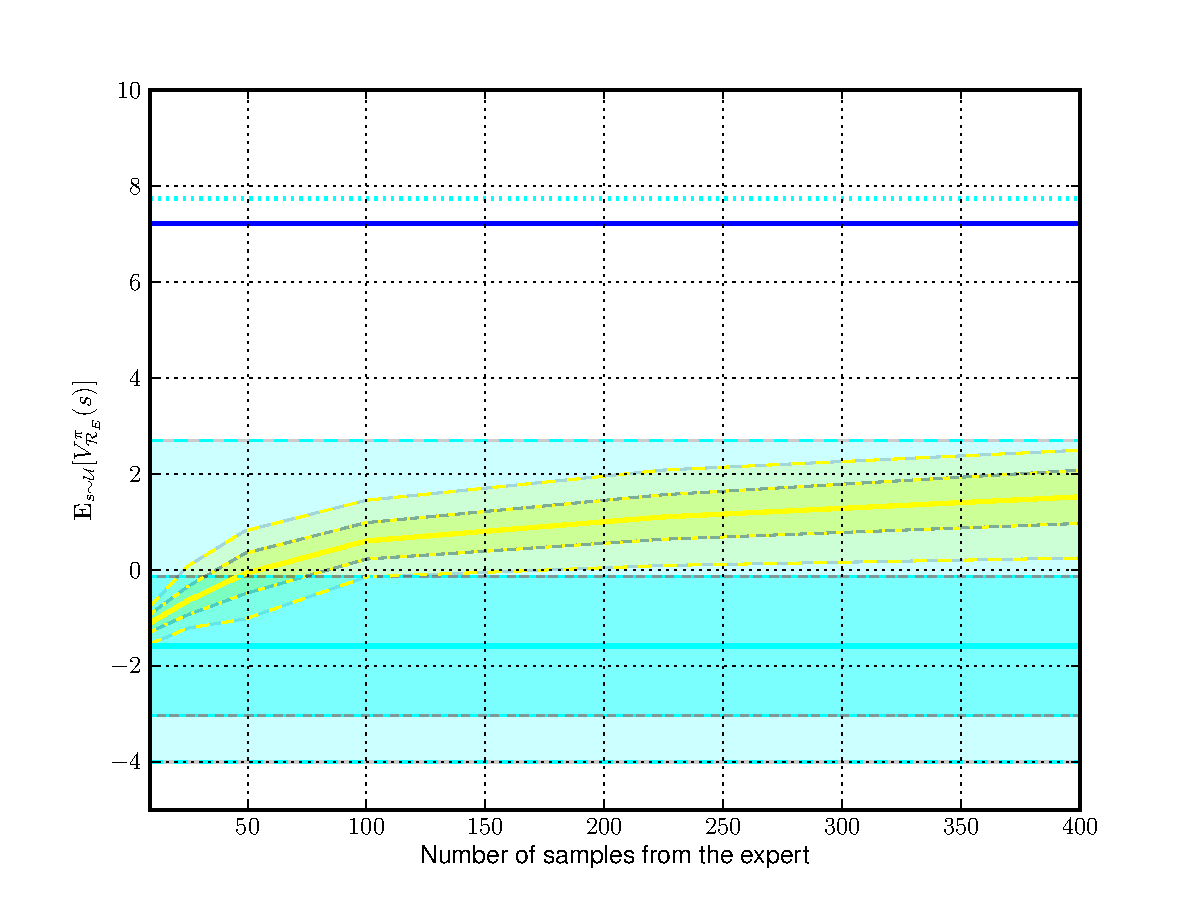
\includegraphics[width=1.2\linewidth]{fig_classif.pdf}}
\end{minipage} \hfill
\begin{minipage}[r]{0.49\linewidth}
\centering
  \centerline{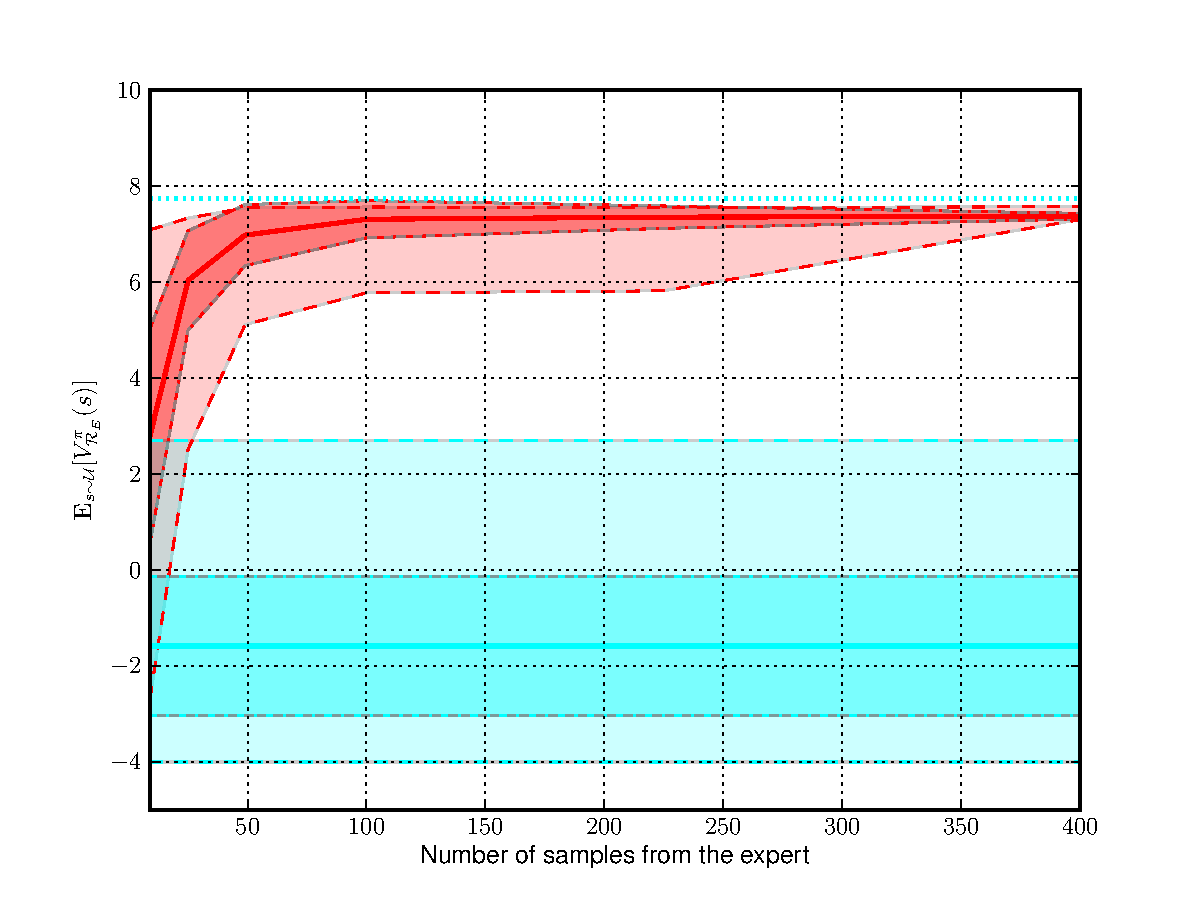
\includegraphics[width=1.2\linewidth]{fig_scirl.pdf}}
\end{minipage}
\end{figure}

La figure~\ref{fies} montre la performance de chacune des approches en fonction du nombre de transitions de l'expert utilisées (sauf pour PIRL qui a utilisé le modèle). On peut voir que le classifieur ne fonctionne pas bien sur ce problème. Augmenter le nombre de transitions améliorerait ses performances, mais après 400 transitions, il ne fonctionne pas aussi bien que SCIRL avec uniquement une dizaine de transitions. Cela illustre la pertinence d'utiliser $\mu$ et non $\phi$ dans la paramétrisation de la fonction de score, l'attribut moyen contient en effet de l’information quant à la dynamique engendrée par la politique de l’expert. SCIRL fonctionne particulièrement bien ici : après seulement une centaine de transitions il atteint les performances de PIRL. Ces deux algorithmes sont proches de la valeur de l'expert. Nous ne fournissons pas de données exactes en ce qui concerne les temps de calcul, mais faire fonctionner SCIRL une fois avec $400$ transitions en entrée est environ une centaine de fois plus rapide que de faire fonctionner PIRL pour $70$ itérations.
%
% (this is due to the need to repeatedly solve MDPs for PIRL).

%Recall that for SCIRL the instantiation of
%section~\ref{subseracticalApproacnstantiation} is considered,
%with a single Monte-Carlo rollout for estimating
%$\hat{\mu}^{\pi_E}(s_i,a_i)$ et using the proposed heuristic for
%$\hat{\mu}^{\pi_E}(s_i,a\neq a_i)$, which goes beyond our analysis.
%To our knowledge, it is the only algorithm working (at least on this
%benchmark) only with data from the expert.


\section{Conclusion}
\label{seonclusion}

Nous avons introduit une nouvelle approche de résolution du problème de l'ARI en structurant un classifieur à fonction de score linéairement paramétrée avec une estimée de l'attribut moyen de l'expert. Il renvoie une fonction de récompense pour laquelle nous avons montré que l'expert est quasi optimal, pour peu que l'erreur de classification soit faible et que l'estimation de l'attribut moyen de l'expert soit bonne. Des méthodes pratiques pour l'estimation de cette grandeur ont été présentées et nous avons introduit une heuristique pour le cas où les seules données disponibles proviennent de l'expert, ainsi qu'une instanciation spécifique de l'algorithme SCIRL. Nous avons exhibé, grâce à un simulateur de conduite sur autoroute, que l'approche proposée fonctionne bien (même combinée à l'heuristique discutée), bien mieux qu'un classifieur non structuré et aussi bien que la méthode de l'état de l'art qui avait accès au modèle (et avec un coût computationnel moindre). Nous prévoyons de poursuivre notre analyse des propritétés théoriques de SCIRL (notamment en vue de l'utilisation avec des heuristiques) et de l'appliquer à des problèmes robotiques réels.

%\acknowledgements{Ces travaux ont été en partie financés par le projet EU FP7 ILHAIRE (Bourse
%n\degree 270780), par le projet EU INTERREG IVa  ALLEGRO et par la Région
%Lorraine (France).}

%\newpage
%\small

\renewcommand\bibname{Bibliographie}
\bibliography{scirl_ria.bib}

\end{document} 
